\section{Rivers \& Streams} \label{sec:rivers_and_streams}

Water networks are essential to the realism of virtual rural terrains. These water networks are constituted of rivers and streams and are the consequence of water being transported by gravity from higher to lower elevation. The algorithm used to model water movement on the terrain is outlined below, along with details concerning the GPU implementation.\\
Unlike work by \cite{Kelley1988} and Št'Ava et al. \cite{StAva2008}, this work does not simulate hydraulic erosion. That is, there is no feedback loop between water movement and the terrain to model changes in terrain relief.

\subsection{Algorithm Overview}

Precipitation, precipitation intensity and soil infiltration are used to calculate the soil humidity, $S_{h}$ (see equation \ref{eq:monthly_soil_humidity}). This equates to the quantity of water, in millimetres, absorbed by the soil. The standing water, \textit{W$_{standing}$}, is the remaining water that is not absorbed by the soil and can be calculated using equation \ref{eq:standing_water_calculation}. \\

\begin{equation} \label{eq:standing_water_calculation}
	W_{standing} = R_{q} - S_{h}
\end{equation}
where:\textit{W$_{standing}$} is the standing water, in millimetres;\textit{R$_{q}$} is the monthly rainfall quantity, in millimetres;\textit{S$_{h}$} is the quantity of water absorbed by the soil, in millimetres.\\

Given the quantity of standing water, W$_{standing}$, for each vertex, a hydrostatic pipe-model similar to that of Stava et al. \cite{StAva2008} is used to determine water movement and build-up on the terrain. This works by iteratively evacuating water from each terrain source vertex \textit{V} to it's eight directly surrounding vertices when possible. The amount of water evacuated to individual surrounding vertices depends on slope and existing water content. During the water evacuation process, Stava et al. \cite{StAva2008} also model the effects of force-based and dissolution-based erosion by modifying the terrain relief depending on calculated forces. This is not simulated in our work however, and the terrain relief remains fixed throughout the simulation. For this reason, our system works best with terrains with pre-existing erosion lines (e.g obtained from real world cartographic data). \\

Although the algorithm is implemented to work in three dimensions where each vertex can evacuate water content to eight surrounding vertices, it also works in a two-dimensional space. With this reduced dimensionality, each vertex \textit{V$_{n}$} has only two neighbouring vertices (\textit{V$_{n-1}$} and \textit{V$_{n+1}$}) in which water can be placed. To better grasp the algorithm, it is described for a two-dimensional space. The concepts are identical when generalised to three dimensions.  \\

Each vertex \textit{V$_{n}$}, is characterised by its position (\textit{n}), terrain height (\textit{TH$_{n}$}), water height (\textit{WH$_{n}$}) and absolute height (\textit{AH$_{n}$} = \textit{TH$_{n}$} + \textit{WH$_{n}$}). Using this data it is possible to calculate the water evacuation capacity, \textit{WEC$_{n}$}, of each terrain vertex (see equation \ref{eq:water_evacuation_capacity}). The value of which effects how much water is evacuated and how it is split amongst surrounding vertices (section \ref{subsec:evacuation_approaches}).

\begin{equation} \label{eq:water_evacuation_capacity}
	WEC_{n} = 2 \times TH_{n} - AH_{n-1} - AH_{n+1}
\end{equation}
Where: \textit{WEC$_{n}$} is the water evacuation capacity of vertex V$_{n}$; \textit{TH$_{n}$} is the terrain height at vertex V$_{n}$, \textit{WH$_{n}$} is the water height at vertex V$_{n}$; \textit{AH$_{n}$} is the absolute height at vertex V$_{n}$.\\

Intuitively, this equation calculates the maximum water quantity which can be evacuated to neighbouring vertices of source vertex \textit{V$_{n}$} whilst ensuring that once the water is added, the aggregate height of these neighbouring vertices does not surpass the terrain height of vertex \textit{V$_{n}$}.\\

\subsection{Water Evacuation Approaches} \label{subsec:evacuation_approaches}

Using the water evacuation capacity \textit{WEC} along with table \ref{tab:scenario_based_on_wec}, one of three evacuation approaches are used:  \textit{all water is evacuated}, \textit{a portion of the water is evacuated} or \textit{no water is evacuated}. Examples scenarios for each approach are illustrated in figure \ref{fig:evacuation_scenarios}. \\

\begin{table}[h]
  \centering
	    \begin{tabular}{|p{6cm}|p{3cm}|p{3cm}|p{3cm}|}
		\hline	
  	     &  WEC $>=$ WaterHeight$_{n}$ & 0 $<$ WEC $<$ WaterHeight$_{n}$ & WEC $<$ 0 \\
  	    \hline	
  	    All water can be evacuated & X & - & - \\
		\hline
  	    A portion of water can be evacuated & - & X & - \\
		\hline
  	    No water can be evacuated & - & - & X \\
		\hline
		\end{tabular}
		\caption{Evacuation approach based on water evacuation capacity (\textit{WEC})}
	  \label{tab:scenario_based_on_wec}
\end{table}

When all water can be evacuated, it is split to surrounding vertices proportionally to their height. This is to model water flowing more intensely on steeper slopes. The quantity of water \textit{W$_{n-1}$} and \textit{W$_{n+1}$} to be evacuated to vertices \textit{V$_{n-1}$} and \textit{V$_{n+1}$} is calculated using equations \ref{eq:all_water_evac_n_minus_one} and \ref{eq:all_water_evac_n_plus_one} . \\

\begin{equation}\label{eq:all_water_evac_n_minus_one}
W_{n-1} = \frac{TerrainHeight_{n} - AbsoluteHeight_{n-1}}{WEC} \times WaterHeight_{n}
\end{equation}

\begin{equation}\label{eq:all_water_evac_n_plus_one}
W_{n+1} = \frac{TerrainHeight_{n} - AbsoluteHeight_{n+1}}{WEC} \times WaterHeight_{n}
\end{equation}

When the water evacuation capacity, \textit{WEC}, does not permit all water to be purged but is sufficient to purge a subset, the amount of water to be evacuated, \textit{W$_{evacuate}$} need to be calculated using equation \ref{eq:evacuate_calc}. \\

\begin{equation}\label{eq:evacuate_calc}
	W_{evacuate} = AbsoluteHeight_{n} - W_{level}
\end{equation}

Where: W$_{level}$ is the water level to which water can be evacuated (see equation \ref{eq:water_level_calc}).

\begin{equation} \label{eq:water_level_calc}
	W_{level} = \frac{AbsoluteHeight_{n-1} + AbsoluteHeight_{n} + AbsoluteHeight_{n+1}}{3}
\end{equation}

When calculated value of \textit{WEC} is less than or equal to zero, no water can be evacuated and therefore no water is purged to neighbouring vertices.

\begin{figure}
\center
	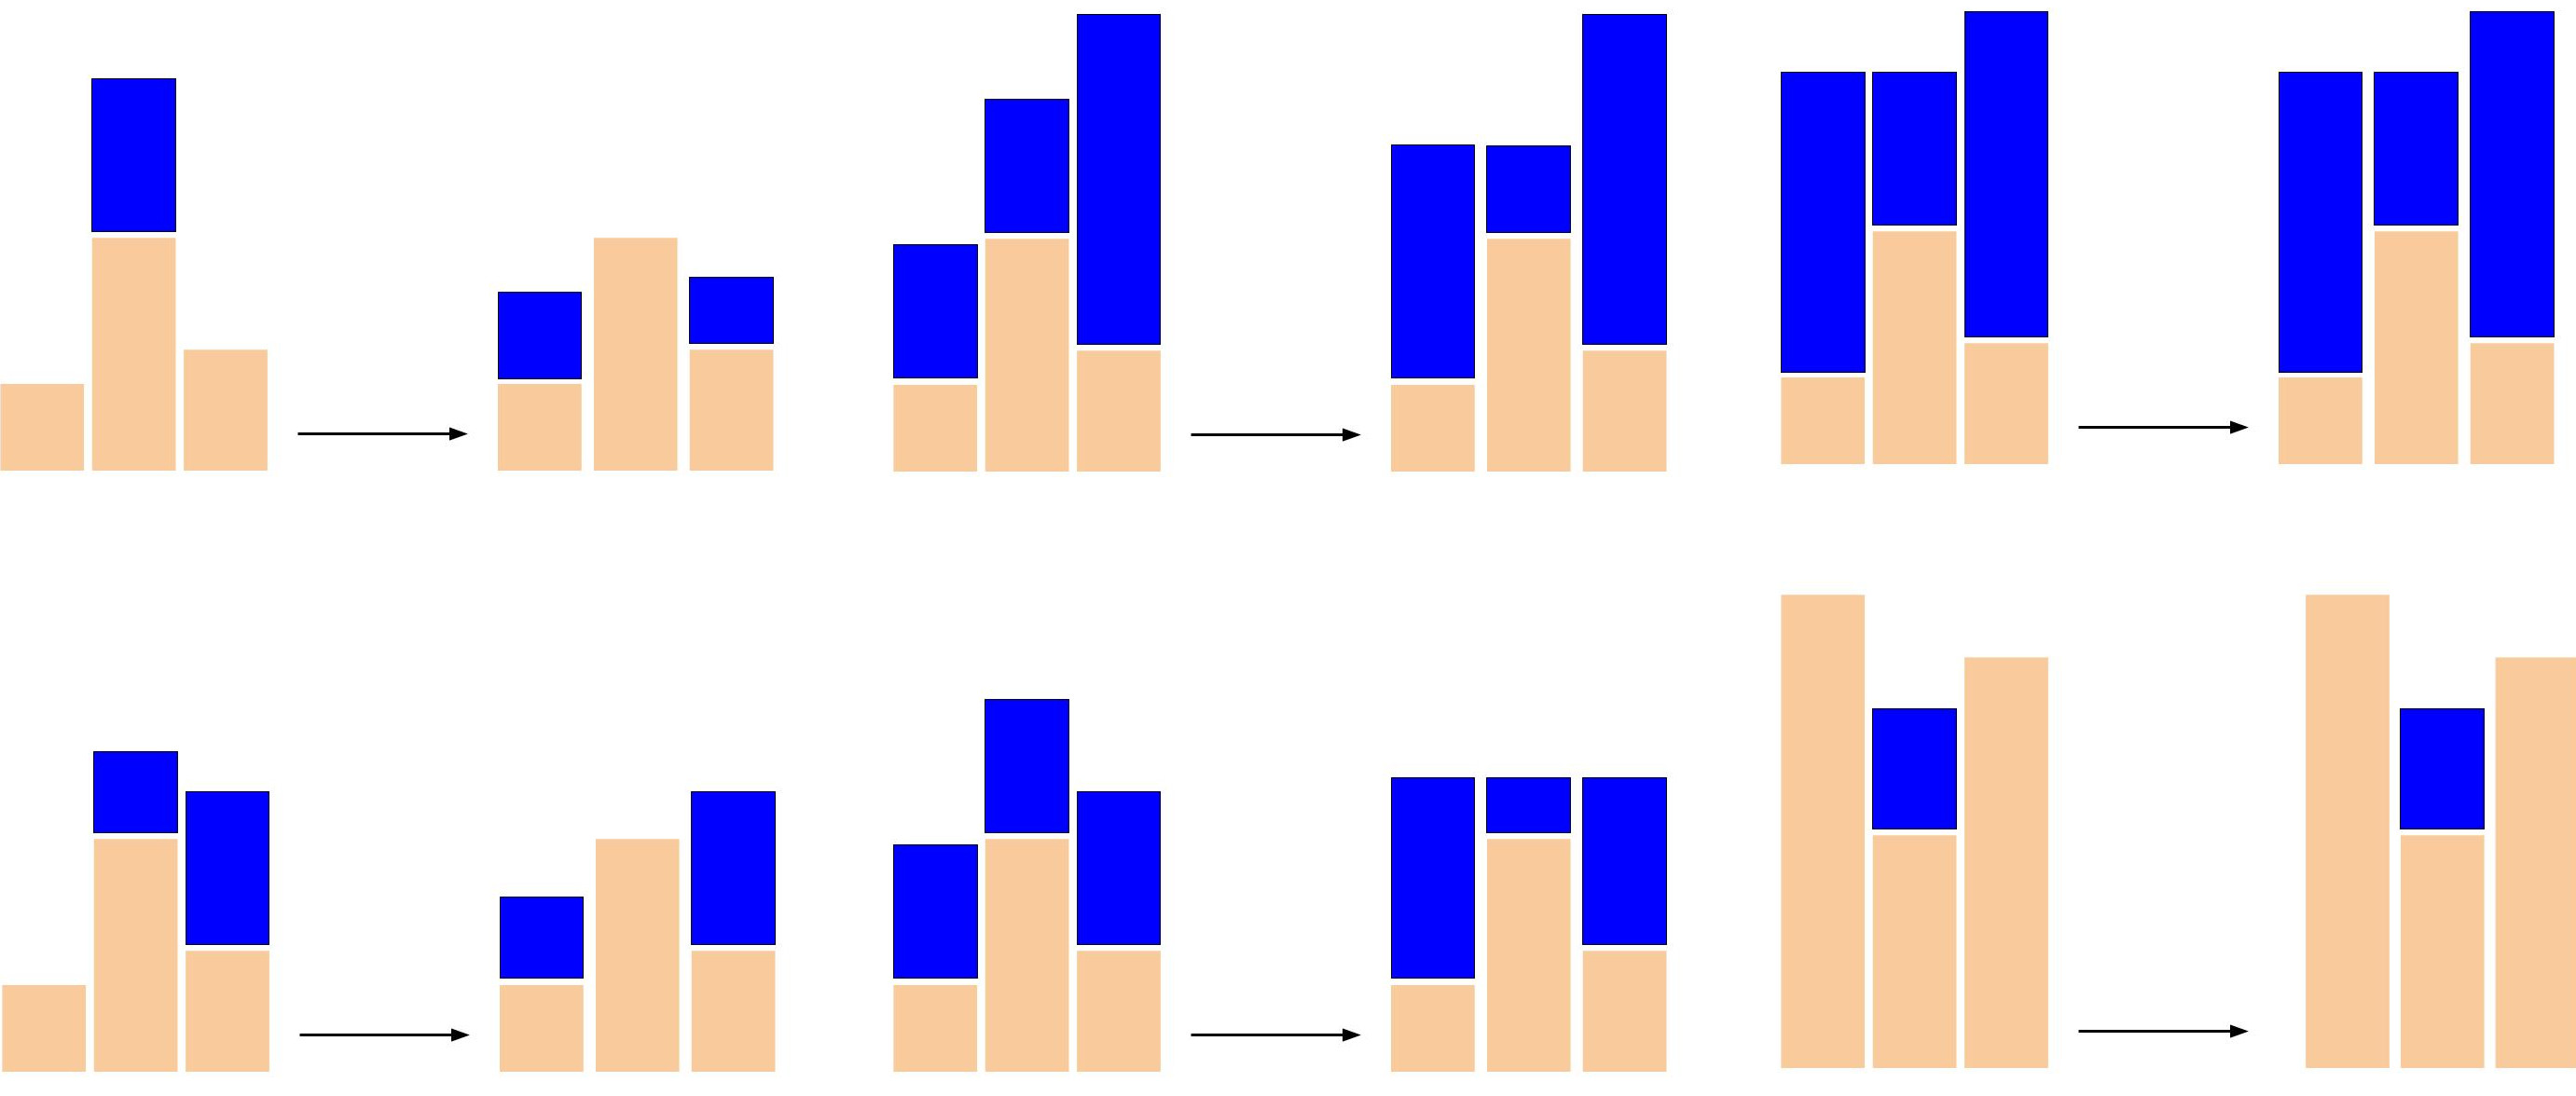
\includegraphics[width=\textwidth]{water_evacuation_all_examples.jpg}
	\caption{ Example water-evacuation scenarios. Left: All water can be evacuated from source vertex (middle). Middle: A portion of water can be evacuated from source vertex (middle). Right: No water can be evacuated from source vertex (middle).}
	\label{fig:evacuation_scenarios}
\end{figure}

\subsection{Terrain Extremities} \label{subsec:terrain_extremeties}

When attempting to evacuate water from vertices on the terrain extremities, one or more vertices will be absent. One way to deal with this would be to discard those vertices and permit water to flow only to existing surrounding vertices. By employing this approach, however, water would never leave the terrain and could build-up unrealistically. To overcome this, a one vertex thick border is generated around the terrain as illustrated in figure \ref{fig:evacuation_border}. The height of each border vertex is calculated such that the slope matches that of it's neighbouring vertices. During the water-flow simulation, water is permitted to evacuate to border vertices but water cannot build-up on them.

\begin{figure}
\center
	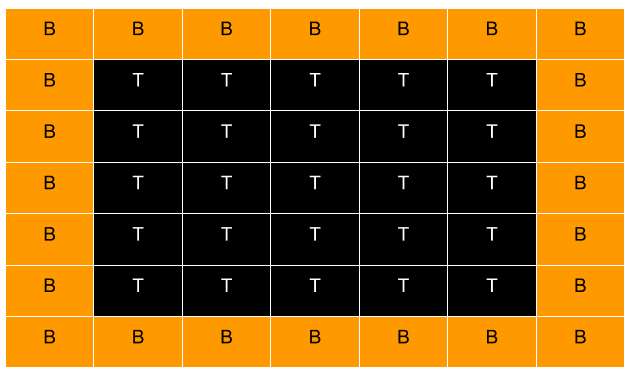
\includegraphics[width=\textwidth/2]{water_evacuation_border.png}
	\caption{ Border of vertices generated around the terrain to cater for water evacuation at the extremities. Orange vertices form the border. }
	\label{fig:evacuation_border}
\end{figure}

\subsection{Stopping the simulation} \label{subsec:stopping_water_flow}

The flow of water on the terrain can be measured by keeping track of the number of vertices that are completely purged at a given iteration of the simulation. This flow will tend to be much larger at the start of the simulation when water is being evacuated from higher ground and will gradually decrease as water starts to build up and less vertices are able to purge their water content entirely. By also keeping track of the aggregated water flow of all previous iterations of the simulation, it is possible to analyse the evolution of water-flow. The system automatically stops the simulation when the water-flow calculated at iteration \textit{n} is less than one thousandth of the total aggregated water which has flowed during the course of the simulation. This value was selected after a large number of trial runs and is deemed conservative as it very often leaves a significant amount of standing water on the terrain. If the user is not satisfied with the formed water network upon completion of the water-flow simulation, he is then able to manually continue the simulation for as long as necessary.

\subsection{GPU Implementation}

Processing water flow on the terrain is computationally expensive as the amount of water to evacuate needs to be calculated iteratively for each terrain vertex. To accelerate the process it is implemented to make use of the heavily parallel architecture of GPU's. \\

GPU's have a single-core multiple thread (SIMT) architecture meaning each operation is performed simultaneously by a large number of threads on different input data. A \textit{work-group} is a grouping of threads within the GPU architecture which are guaranteed to run in parallel and which share local memory with very fast access speeds. One or more work-groups can execute at the same time.\\

Below are discussed the challenges faced when implementing the water-flow algorithm to run on this heavily parallel architecture.

Copying data from CPU to GPU and vice versa is a costly process and, if substantial, can often be the bottleneck to the GPU optimisation. To prevent this, all data is copied to the GPU at the start of the simulation and only when the simulation is complete is the resulting data copied back to the CPU. The only piece of data which is copied back to the CPU between each iteration of the simulation is the aggregated water-flow in order to automatically stop the simulation when suited (see \ref{subsec:stopping_water_flow}).\\

To better fit into the \textit{openGL} pipeline used in this system, GPU implementations are done using \textit{compute shaders}. Compute shaders are a feature of \textit{openGL} since version 4.3 and permit the use the GPU's acceleration potential for tasks not directly linked to rendering. One of the main incentives to use compute shaders is the ability to use existing openGL data storages, notably pre-existing height-map and water-height textures used for rendering. Table \ref{tab:water_flow_simul_mem_allocs} summarizes the global memory allocations necessary for the GPU implementation of the water-flow simulation.\\

\begin{table}[]
  \centering
	    \begin{tabular}{|p{3cm}|p{1.5cm}|p{6cm}|p{5cm}|}
		\hline	
  	    \textbf{Storage Type} &  \textbf{Data Type} & \textbf{Element Count} & \textbf{Usage} \\
		\hline
		2-D Texture & Float & W $\times$ H & Water height-map\\
		\hline
		2-D Texture & Float & W $\times$ H & Cached water height-map from previous iteration in order to calculate the water-flow\\
		\hline
		2-D Texture & Float & (W+1) $\times$ (H+1) & Terrain height-map with border (see \ref{subsec:terrain_extremeties}) \\
		\hline
		2-D Texture & Float & $ W \times GroupCount_{y} \times 2 $ & Horizontal overlaps  \\
		\hline
		2-D Texture & Float & $ GroupCount_{x} \times 2 \times H $ & Vertical overlaps  \\
		\hline
		2-D Texture & Float & $ 4 \times GroupCount_{x} \times GroupCount_{y}$ & Corner overlaps  \\
		\hline
		2-D Texture & Unsigned int & $ GroupCount_{x} \times GroupCount_{y}$ & Water flow tracker \\
		\hline
		\end{tabular}
		\caption{Global memory allocations necessary for the GPU implementation of the water-flow simulation algorithm where \textit{W} and \textit{H} are the width and height of the terrain height-map respectively.}
	  \label{tab:water_flow_simul_mem_allocs}
\end{table}

Each thread within a work-group relates to a unique vertex on the terrain from which water must be evacuated. Water evacuated from source vertex must be added to one or many of its eight surrounding vertex/vertices by incrementing it's value within the water height-map data structure. Memory conflicts can arise, however, when multiple threads attempt to evacuate water to the same location within this water height-map. Given a destination location \textit{D}, up to eight threads can attempt to write to it simultaneously (see figure \ref{fig:water_flow_dest_conflicts}).\\ 

\begin{figure}
\center
	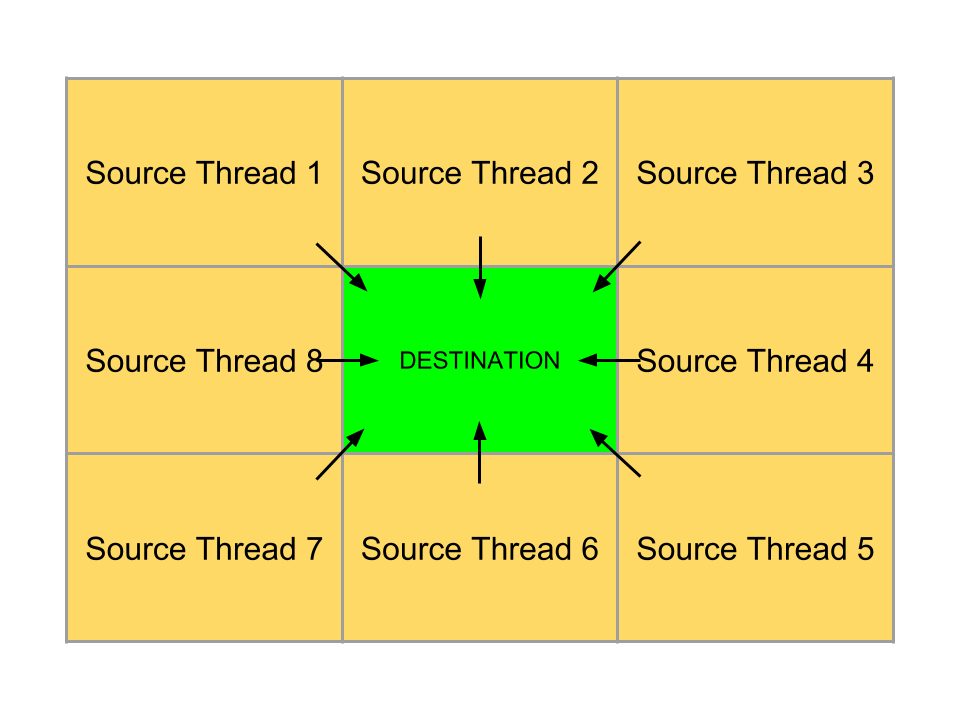
\includegraphics[width=\textwidth]{water_flow_dest_conflicts.png}
	\caption{ Memory conflict cause by 8 surrounding threads attempting to write to a single destination memory location. }
	\label{fig:water_flow_dest_conflicts}
\end{figure}

To prevent such memory conflicts, a temporary three-dimensional array is allocated in local storage (fast-access) for each work group in which water movement is written. The x and y dimensions of this temporary array are the width and height of the associated work-group respectively and each [x,y] pair represent a unique destination on the terrain in which water can be added. The third-dimension serves to prevent memory conflicts by giving each source vertex a unique index in which to write water to add (see figure\ref{fig:water_flow_dest_conflict_prevent}).\\

\begin{figure}
\center
	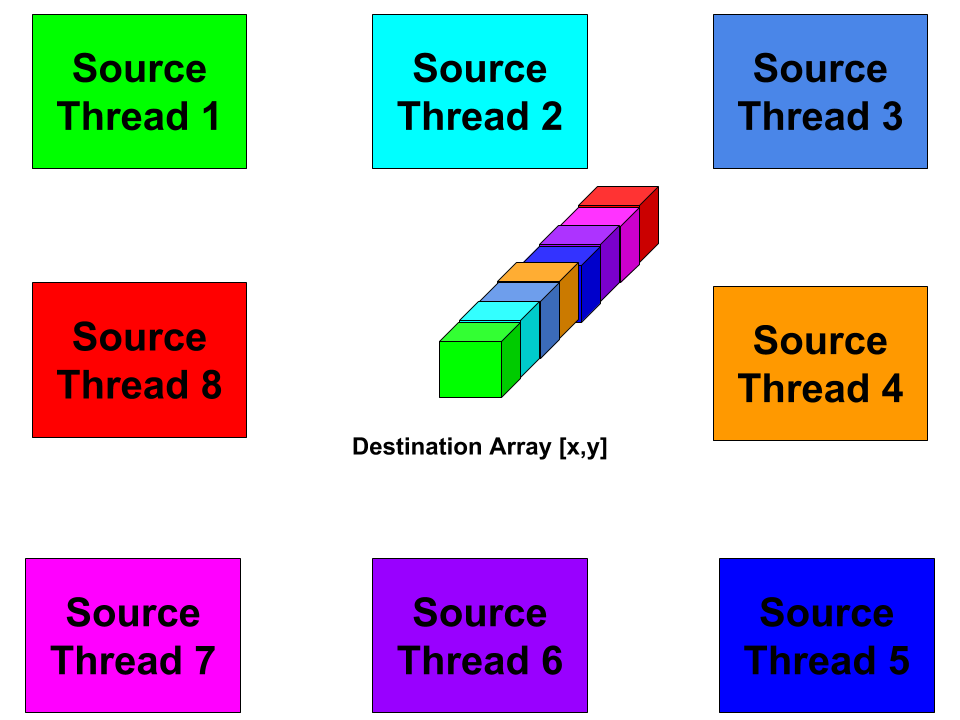
\includegraphics[width=\textwidth]{water_flow_memory_conflict_prevention.png}
	\caption{ Memory conflict prevention by using a three dimensional array to aggregate the water to add. }
	\label{fig:water_flow_dest_conflict_prevent}
\end{figure}

When water movement is complete for the given iteration, each thread \textit{T$_{xy}$} within a work group reduces the third dimension of it's associated aggregate array index [x,y] by adding all values to the respective location within the water height-map.\\

Because local memory cannot be shared amongst work-groups, a problem arises when threads on the extremities need to place water on vertices managed by threads from a separate work-group. A work group \textit{WG$_{xy}$} at index [x,y] may need access to neighbouring work groups in the horizontal direction (figure \ref{fig:water_flow_inter_wg_reduc_horiz}), vertical direction (figure \ref{fig:water_flow_inter_wg_reduc_vert}) and diagonal direction (figure \ref{fig:water_flow_inter_wg_reduc_diag}). Global memory is allocated (2-D textures) to aggregate the data to be written to these locations. When water-flow for the given iteration is complete, this data is then reduced by selected threads and written back to the water height-map.

\begin{figure}
\center
	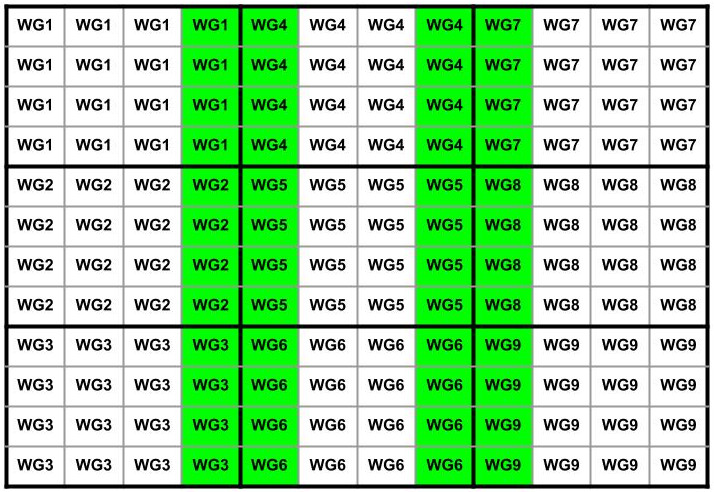
\includegraphics[width=\textwidth/2]{inter_work_group_reduction_textures_horizontal.jpg}
	\caption{ Global memory allocation requirement (green) to cater for inter work group memory access in the horizontal direction. \textit{WG} = work group}
	\label{fig:water_flow_inter_wg_reduc_horiz}
\end{figure}

\begin{figure}
\center
	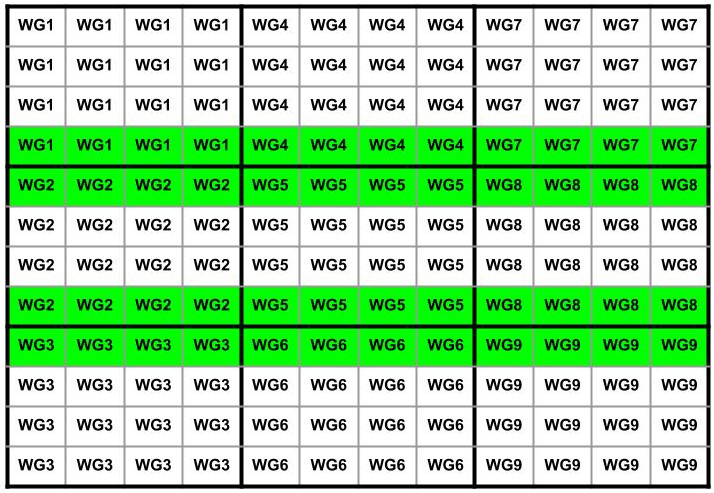
\includegraphics[width=\textwidth/2]{inter_work_group_reduction_textures_vertical.jpg}
	\caption{ Global memory allocation requirement (green) to cater for inter work group memory access in the vertical direction. \textit{WG} = work group}
	\label{fig:water_flow_inter_wg_reduc_vert}
\end{figure}

\begin{figure}
\center
	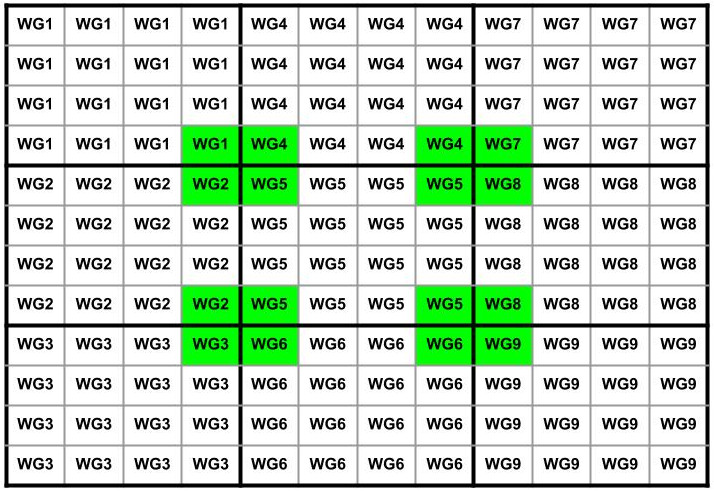
\includegraphics[width=\textwidth/2]{inter_work_group_reduction_textures_diagonal.jpg}
	\caption{ Global memory allocation requirement (green) to cater for inter work group memory access in the diagonal direction. \textit{WG} = work group}
	\label{fig:water_flow_inter_wg_reduc_diag}
\end{figure}

\subsection{Performance}

Due to limited scope, a CPU version of this algorithm was not implemented and therefore, calculating GPU speed-up is not possible. The section focuses on the processing time to complete the water-flow simulation and the average time per single-iteration of the simulation for terrains varying in size. \\
In order to ensure consistency between the tests:
\begin{itemize}
\item The different terrains used are all scaled-down versions of the same seed terrain. This ensures the terrain relief, and therefore water-flow capacity, is the same.\\
\item The amount of water to evacuate at time \textit{t$_{0}$} on each terrain vertex is the same for all simulation runs (100 millimetres). \\
\end{itemize}

As can be seen in the results summarised in figure \ref{fig:water_flow_processing_time_total}, the water-flow simulation takes approximately 22 seconds to complete for a terrain with over one million vertices (1024 $\times$ 1024 terrain). The simulation time decreases linearly with the vertex count of the terrain. A similar pattern emerges when analysing the average processing time for a single iteration of the simulation (see figure \ref{fig:water_flow_processing_time_per_iteration}).

\begin{figure}
\center
	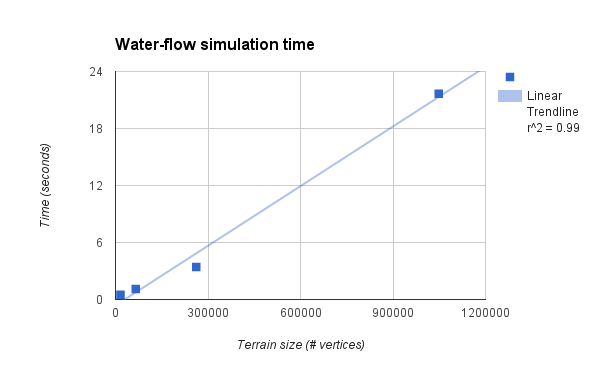
\includegraphics[width=\textwidth]{water_flow_processing_time_total.png}
	\caption{ Total water-flow simulation time for 100 millimetres per terrain vertex. Analysis performed for terrains with dimensions: 128 by 128, 256 by 256, 512 by 512 and 1024 by 1024.}
	\label{fig:water_flow_processing_time_total}
\end{figure}

\begin{figure}
\center
	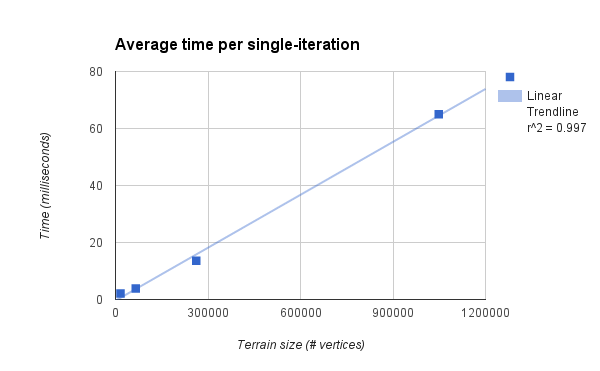
\includegraphics[width=\textwidth]{water_flow_processing_time_per_iteration.png}
	\caption{ Average time for a single iteration of the water-flow for 100 millimetres per terrain vertex. Analysis performed for terrains with dimensions: 128 by 128, 256 by 256, 512 by 512 and 1024 by 1024.}
	\label{fig:water_flow_processing_time_per_iteration}
\end{figure}

\subsection{Results}

The U.S. Geological Survey \protect\footnotemark \footnotetext{\url{http://www.usgs.gov}}  freely provides detailed elevation data for the north American continent. Also, Google-Earth \protect\footnotemark \footnotetext{\url{http://www.google.com/earth/}} provides detailed satellite images of the same locations. To test the water-flow simulation, we use terrains downloaded from the U.S. Geological Survey. The resulting rivers and streams which are then compared with corresponding satellite images to see if the main water bodies match. For the tests to be as accurate as possible, only the water-flow simulation is performed on the terrains with not fine-tuning of soil infiltration rates. \\
The results illustrated in figures \ref{fig:water_flow_test_1}, \ref{fig:water_flow_test_2} and \ref{fig:water_flow_test_3} show that the simulation successfully reproduces core water networks. Note that the replicated terrains also contain water bodies and rivers which are not present in the corresponding satellite image. The purpose of the test is not to reproduce an exact match but rather ensure that, by running only the water-flow simulation, the core water networks are reproduced. Better results could be achieved by fine-tuning the soil infiltration rates but this would bias the test as it would influence the flow of water on the terrain.

An important simplification worth noting of the water-flow simulation is that water absorption is not performed whilst it is running. In other words, when water is evacuated from source to destination vertex, no water is then absorbed in the destination vertex. Integrating secondary absorption into the simulation would improve realism as not only would it improve the accuracy of standing water but also of the vegetation as it would lead to more precise soil humidities. This would expensive, however, as similarly to the work by Lau \cite{Lau2010} it would require the calculation of water flow velocities based on relief and soil properties. Because of scope, it was not possible to incorporate this into this water-flow simulation but would form a valuable addition in future work. As shown in the tests below, however, this simulation is still extremely valuable in determining where river networks form on the terrain.

\begin{figure}
\center
	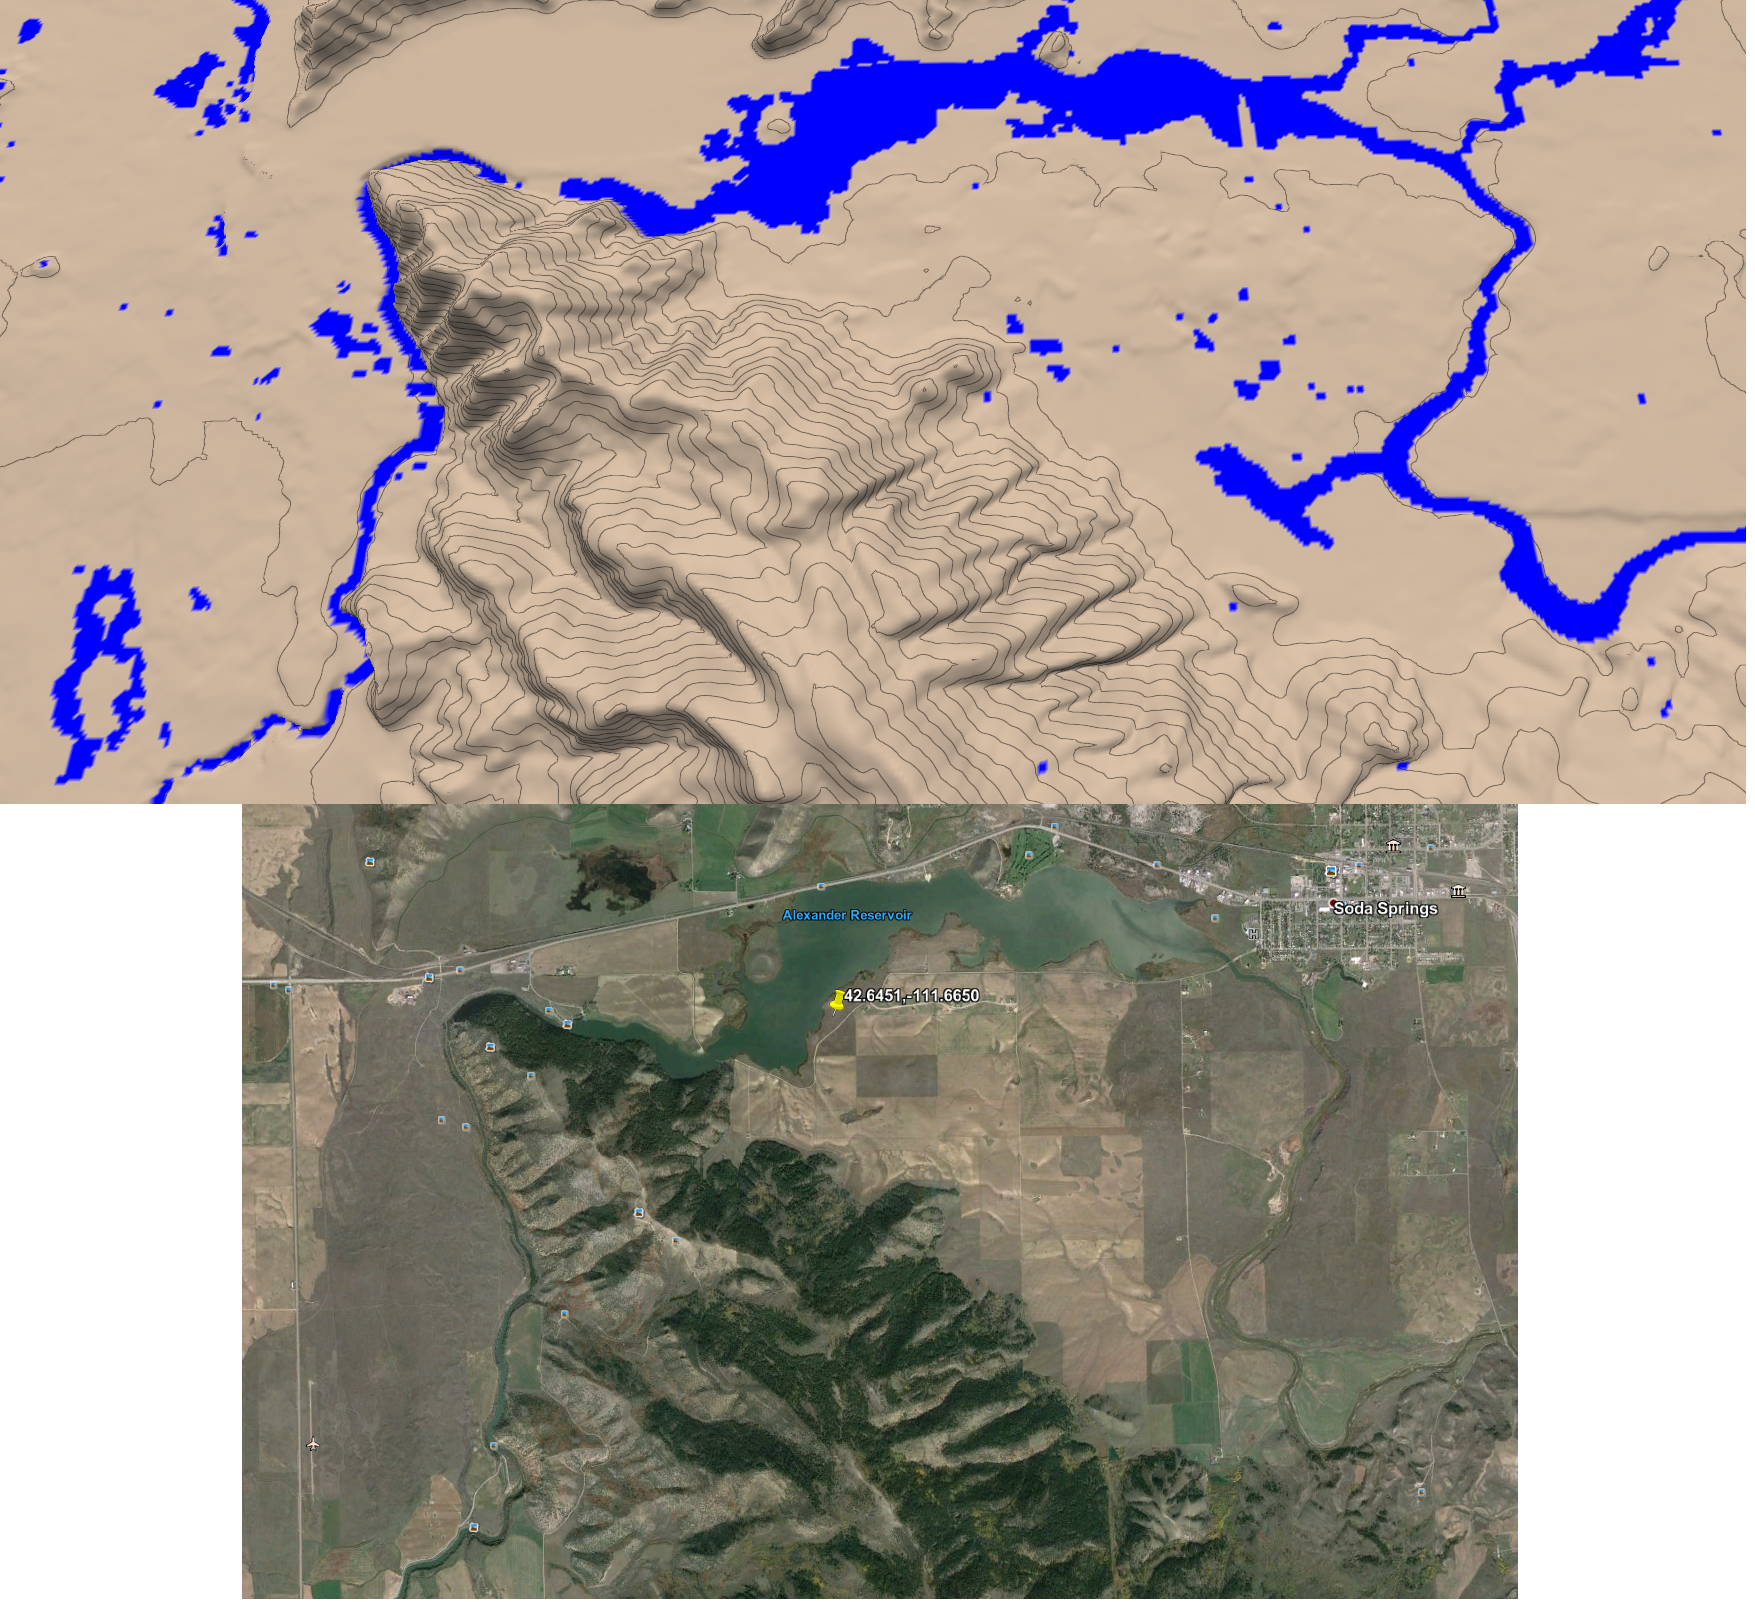
\includegraphics[width=\textwidth]{water_flow_test_1.png}
	\caption{ Top: Real world water-network at geographic coordinate location: 42\textdegree38'N 111\textdegree35'W. Bottom: Replica using the water-flow simulation.}
	\label{fig:water_flow_test_1}
\end{figure}

\begin{figure}
\center
	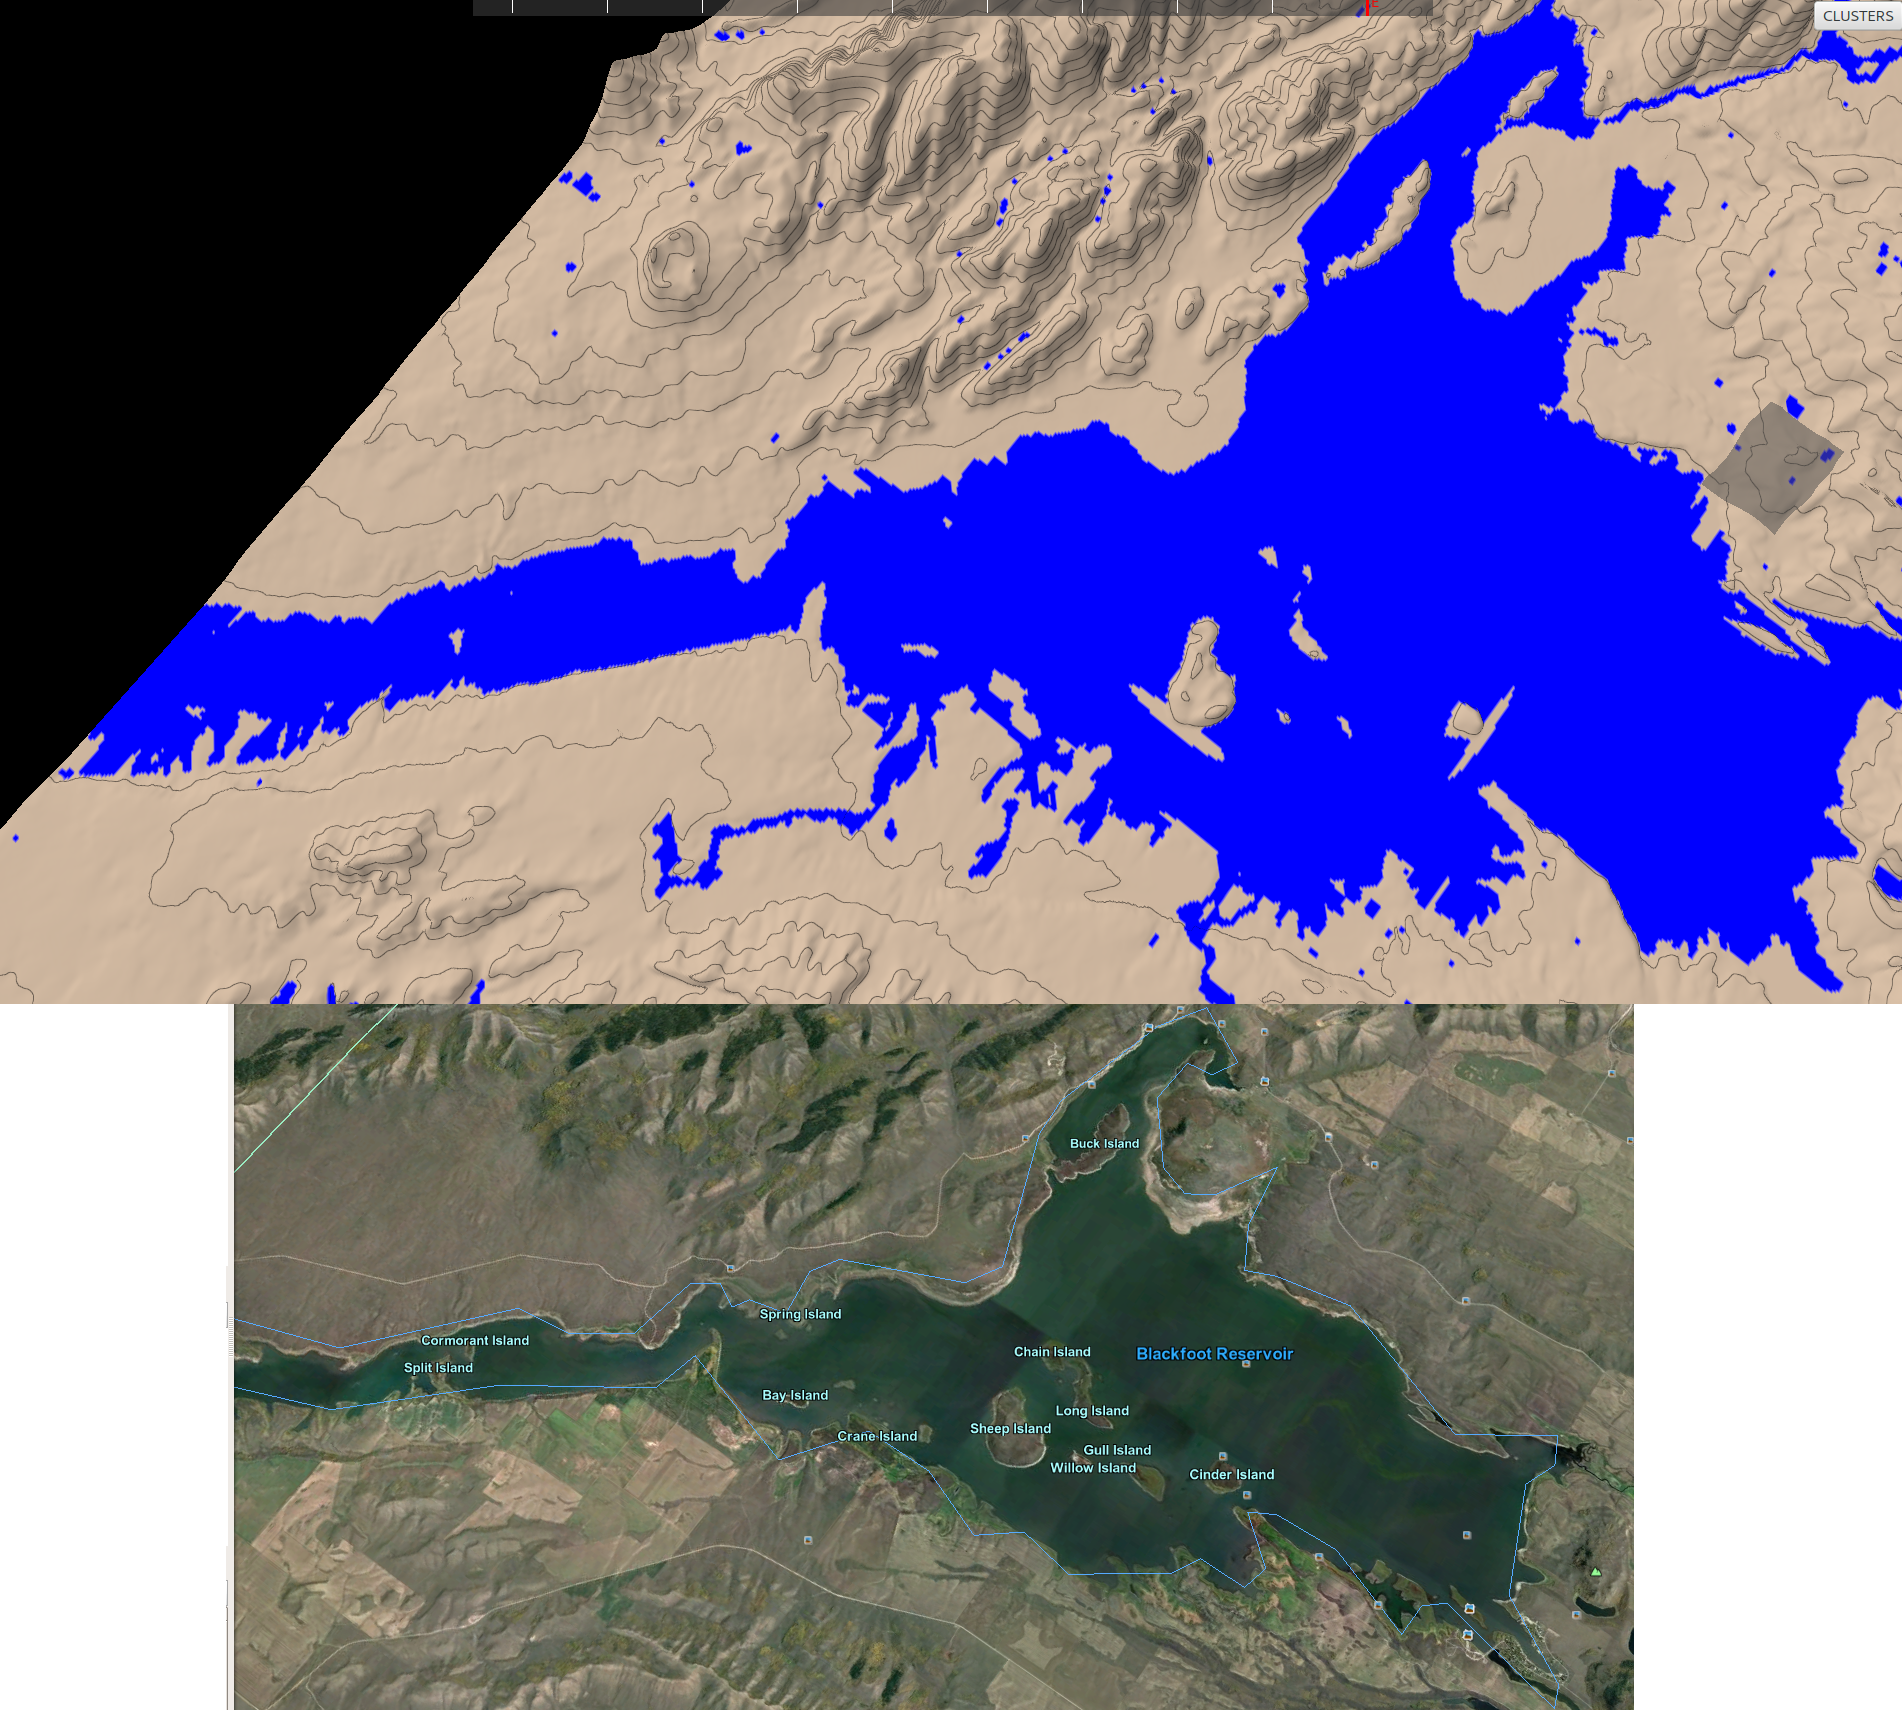
\includegraphics[width=\textwidth]{water_flow_test_2.png}
	\caption{ Top: Real world water-network at geographic coordinate location: 49\textdegree39'N 116\textdegree52'W. Bottom: Replica using the water-flow simulation.}
	\label{fig:water_flow_test_2}
\end{figure}

\begin{figure}
\center
	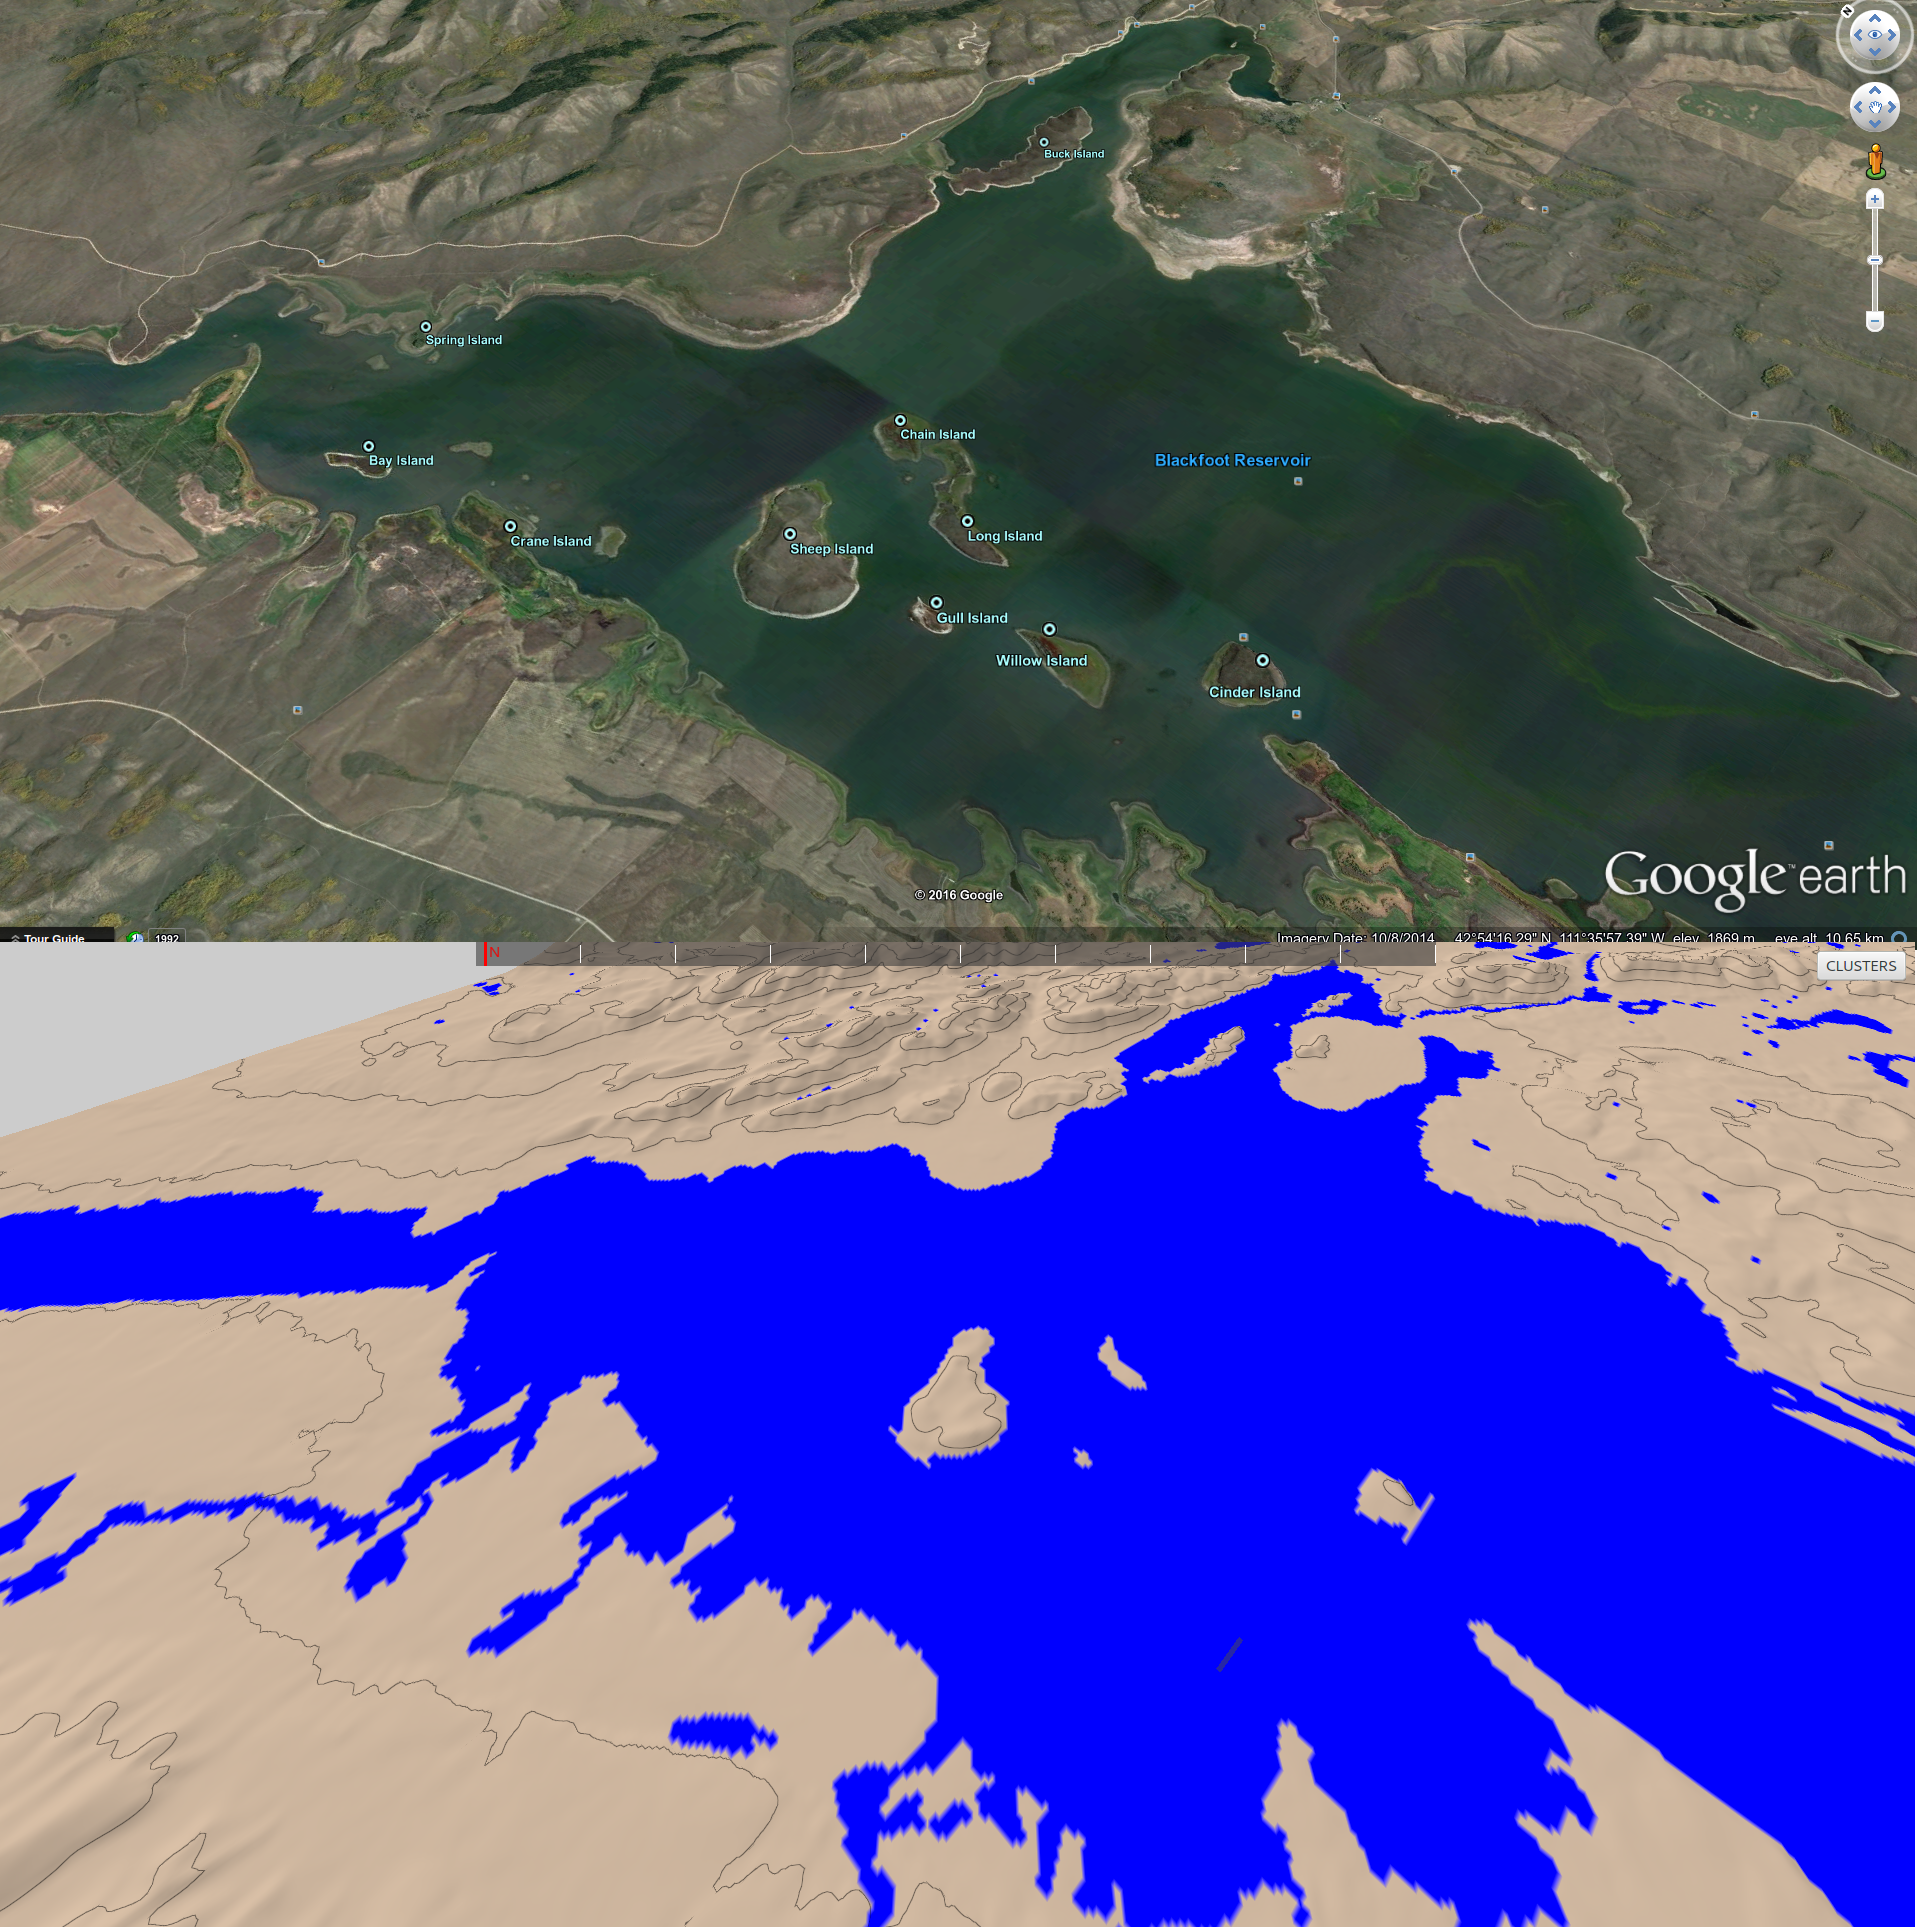
\includegraphics[width=\textwidth]{water_flow_test_3.png}
	\caption{ Top: Real world water-network at geographic coordinate location: 42\textdegree38'N 111\textdegree35'W. Bottom: Replica using the water-flow simulation.}
	\label{fig:water_flow_test_3}
\end{figure}